% ======================================================

\begin{frame}{Non-Uniform Grids (1/)}
\begin{itemize}
    \item \textbf{Problem} - cannot achieve a uniform distribution of discretization error on a uniform grid.
    \item \textbf{Solution} - use a smaller $\Delta x$ in regions where the derivatives of the function is large, and a larger $\Delta x$ when the function is smooth.
    \item \textbf{Aim} - spread the error nearly uniformly over the domain.
\end{itemize} 
\end{frame}

% ======================================================

\begin{frame}{Non-Uniform Grids (2/)}
\begin{itemize}
    \item Truncation error for the CDS is     
    \[
    \epsilon_{r} = 
    - \frac{(\Delta x_{i+1})^{2} - (\Delta x_{i})^{2}}{2(x_{i+1}-x_{i-1})}\bigg(\frac{\partial^{2} \phi}{\partial x^{2}}\bigg)_{i} + \frac{(\Delta x_{i+1})^{3} + (\Delta x_{i})^{3}}{6(x_{i+1}-x_{i-1})}\bigg(\frac{\partial^{3} \phi}{\partial x^{3}}\bigg)_{i} + H
    \]
    where $\Delta x_{i+1} = (x_{i+1}-x_{i})$ and $\Delta x_{i} = (x_{i}-x_{i-1})$. 
    
    \item \textbf{Assume} the grid expands or contracts with a constant factor $r_{e}$, known as a compound interest grid, we have: \[\Delta x_{i+1} = r_{e}\Delta x_{i}\]
    
    \item \textbf{Therefore}, the leading truncation error:
    \begin{itemize}
        \item For CDS: 
        \[
        \epsilon_{r} \approx
        \frac{(1-r_{e})\Delta x_{i}}{2}\bigg(\frac{\partial^{2}\phi}{\partial x^{2}}\bigg)_{i}
        \]
        \item For FDS and BDS (first-order):
        \[
        \epsilon_{r} \approx
        \frac{\Delta x_{i}}{2}\bigg(\frac{\partial^{2}\phi}{\partial x^{2}}\bigg)_{i}
        \]
    \end{itemize}
\end{itemize}
\end{frame}
%%=======================================================
\begin{frame}{Non-Uniform Grids (3/)}
 The leading truncation error:
    \begin{itemize}
        \item For CDS: 
        \[
        \epsilon_{r} \approx
        \frac{(1-r_{e})\Delta x_{i}}{2}\bigg(\frac{\partial^{2}\phi}{\partial x^{2}}\bigg)_{i}
        \]
        \item For FDS and BDS (first-order):
        \[
        \epsilon_{r} \approx
        \frac{\Delta x_{i}}{2}\bigg(\frac{\partial^{2}\phi}{\partial x^{2}}\bigg)_{i}
        \]
    \end{itemize}
From above, as $r_{e}$ is close to unity, the first-order truncation error of the CDS is substantially smaller than the FDS/BDS error.
\end{frame}
%%=======================================================
\begin{frame}{Non-Uniform Grids (4/)}
\begin{itemize}
    \item \textbf{Q:} what will happen when the grid is refined?
    \item Consider two scenarios: (1)\textbf{halving the spacing between two coarse grids} and (2)\textbf{inserting new points with a constant ratio of spacing}.
\end{itemize}
    
\metroset{block=fill}
\begin{block}{Scenario 1: halving the space}
    The spacing is uniform around new points with a constant $r_{e}$. If we repeat the refinement for several times, we can obtain a grid with uniform spacing \textit{almost} everywhere, except near the two coarsest points. Therefore, the CDS error vanishes.
\end{block}
\end{frame}
%%=======================================================
\begin{frame}[fragile]{Non-Uniform Grids (5/)}
\begin{figure}
    \centering
    \includegraphics[width=\textwidth]{imgs/non-uniform.eps}
    \caption{Refinement of a non-uniform grid}
    \label{fig:non-uniform}
\end{figure}

\metroset{block=fill}
\begin{block}{Scenario 2: inserting new points}\small
The expansion factor of the fine grid is smaller than on the coarse grid: $r_{e, h} = \sqrt{r_{e, 2h}}$, where $h$ represents the refined grid, and $2h$, the coarse grid. The ratio of the leading truncation error term at node $i$ on the two grids is:
    \[
    r_{\tau} = \frac{(1-r_{e})_{2h}(\Delta x_{i})_{2h}}{(1-r_{e})_{h}(\Delta x_{i})_{h}}
    \]
From \autoref{fig:non-uniform}:
    \[
    (\Delta x_{i})_{2h} = (\Delta x_{i})_{h} + (\Delta x_{i-1})_{h} = (r_{e}+1)_{h}(\Delta x_{i-1})_{h}
    \]
\end{block}
\end{frame}

%%=======================================================
\begin{frame}[fragile]{Non-Uniform Grids (6/)}
\metroset{block=fill}
\begin{block}{Scenario 2: inserting new points - CONT'D}\small
From \autoref{fig:non-uniform}:
    \[
    (\Delta x_{i})_{2h} = (\Delta x_{i})_{h} + (\Delta x_{i-1})_{h} = (r_{e}+1)_{h}(\Delta x_{i-1})_{h}
    \]
Therefore, the first-order truncation error of the CDS is reduced by a factor 
    \[
    r_{\tau} = \frac{(1+r_{e,h})^{2}}{r_{e,h}}
    \]
    When $r_{e} =1$, \textit{i.e.} when the grid is uniform, the factor $r_{\tau} = 4$; When $r_{e} < 1$ or $r_{e} > 1$, \textit{i.e.} the grid is contacting or expanding, the factor $r_{\tau}>4$. This means that the error due to the first-order term decreases faster than the second-order error term.
\end{block}
\textbf{Conclusion:} systematic refinement of non-uniform grids gives a rate of reduction of truncation error that has the same order as for a uniform gird.
\end{frame}

%%=======================================================
\begin{frame}[fragile]{Non-Uniform Grids (7/)}
\metroset{block=fill}
Higher order approximation of the first derivative can be obtained by using more points to eliminate more of the truncation error terms. For example, using $\phi_{i-1}$ to obtain an expression for the second derivative at $x_{i}$:
    \begin{align*}
    \bigg( \frac{\partial \phi}{\partial x} \bigg)_{i} 
    & = \frac{\phi_{i+1}(\Delta x_{i})^{2}-\phi_{i-1}(\Delta x_{i+1})^{2} + \phi_{i}[(\Delta x_{i+1})^{2}-(\Delta x_{i})^{2}]}{\Delta x_{i+1}\Delta x_{i}(\Delta x_{i}+\Delta x_{i+1})} \\
    & - \frac{\Delta x_{i+1}\Delta x_{i}}{6}\bigg( \frac{\partial^{3} \phi}{\partial x^{3}} \bigg)_{i} + H
    \end{align*}
\end{frame}
